%%%%%%%%%%%%%%%%%%%%%%%%%%%%%%%%%%%%%%%%%
% Beamer Presentation
% LaTeX Template
% Version 1.0 (10/11/12)
%
% This template has been downloaded from:
% http://www.LaTeXTemplates.com
%
% License:
% CC BY-NC-SA 3.0 (http://creativecommons.org/licenses/by-nc-sa/3.0/)
%
%%%%%%%%%%%%%%%%%%%%%%%%%%%%%%%%%%%%%%%%%

%----------------------------------------------------------------------------------------
%	PACKAGES AND THEMES
%----------------------------------------------------------------------------------------

\documentclass{beamer}

\mode<presentation> {

% The Beamer class comes with a number of default slide themes
% which change the colors and layouts of slides. Below this is a list
% of all the themes, uncomment each in turn to see what they look like.

%\usetheme{default}
%\usetheme{AnnArbor}
%\usetheme{Antibes}
%\usetheme{Bergen}
%\usetheme{Berkeley}
%\usetheme{Berlin}
%\usetheme{Boadilla}
%\usetheme{CambridgeUS}
%\usetheme{Copenhagen}
%\usetheme{Darmstadt}
%\usetheme{Dresden}
%\usetheme{Frankfurt}
%\usetheme{Goettingen}
%\usetheme{Hannover}
%\usetheme{Ilmenau}
%\usetheme{JuanLesPins}
%\usetheme{Luebeck}
\usetheme{Madrid}
%\usetheme{Malmoe}
%\usetheme{Marburg}
%\usetheme{Montpellier}
%\usetheme{PaloAlto}
%\usetheme{Pittsburgh}
%\usetheme{Rochester}
%\usetheme{Singapore}
%\usetheme{Szeged}
%\usetheme{Warsaw}

% As well as themes, the Beamer class has a number of color themes
% for any slide theme. Uncomment each of these in turn to see how it
% changes the colors of your current slide theme.

%\usecolortheme{albatross}
%\usecolortheme{beaver}
%\usecolortheme{beetle}
%\usecolortheme{crane}
%\usecolortheme{dolphin}
%\usecolortheme{dove}
%\usecolortheme{fly}
%\usecolortheme{lily}
%\usecolortheme{orchid}
%\usecolortheme{rose}
%\usecolortheme{seagull}
%\usecolortheme{seahorse}
%\usecolortheme{whale}
%\usecolortheme{wolverine}

%\setbeamertemplate{footline} % To remove the footer line in all slides uncomment this line
%\setbeamertemplate{footline}[page number] % To replace the footer line in all slides with a simple slide count uncomment this line

%\setbeamertemplate{navigation symbols}{} % To remove the navigation symbols from the bottom of all slides uncomment this line
}
\usepackage{comment}
\usepackage{graphicx} % Allows including images
\usepackage{booktabs} % Allows the use of \toprule, \midrule and \bottomrule in tables

%----------------------------------------------------------------------------------------
%	TITLE PAGE
%----------------------------------------------------------------------------------------

\title[Antenna Simulations]{Simulations of dipole and array antennas in MATLAB} % The short title appears at the bottom of every slide, the full title is only on the title page

\author{Marika Svensson} % Your name
\institute[Signals and Systems] % Your institution as it will appear on the bottom of every slide, may be shorthand to save space
{
Chalmers University of Technology \\ % Your institution for the title page
\medskip
\textit{marikasvenssonplepla@gmail.com} % Your email address
}
\date{\today} % Date, can be changed to a custom date

\begin{document}

\begin{frame}
\titlepage % Print the title page as the first slide
\end{frame}

\begin{frame}
\frametitle{Overview} % Table of contents slide, comment this block out to remove it
\tableofcontents % Throughout your presentation, if you choose to use \section{} and \subsection{} commands, these will automatically be printed on this slide as an overview of your presentation
\end{frame}

%----------------------------------------------------------------------------------------
%	PRESENTATION SLIDES
%----------------------------------------------------------------------------------------

%------------------------------------------------
\section{Task 1-6} % Sections can be created in order to organize your presentation into discrete blocks, all sections and subsections are automatically printed in the table of contents as an overview of the talk
%------------------------------------------------
\subsection{Theory and results}
\subsection{Dipole antenna} % A subsection can be created just before a set of slides with a common theme to further break down your presentation into chunks
\subsection{Irregular and equispaced antennas}

%------------------------------------------------
\begin{frame}
\frametitle{Task 1: Theory}
If the dipole is considered to be short
\begin{equation}
\mathbf{G}(\theta, \phi) = G_{\theta}\hat{\theta} + G_{\phi}\hat{\phi},
\end{equation}
with

\begin{equation}
\begin{cases}
&G_{\theta} = G_{\theta}(\theta, \phi) = C_k\eta I_0 l/2cos(\theta)sin(\phi)2jsin(khcos(\theta))) \\
& G_{\phi} = G_{\phi}(\theta, \phi) = C_k\eta I_0 l/2cos(\phi)2jsin(khcos(\theta))).
\end{cases}
\end{equation} 
with 
\begin{equation}
\begin{cases}
& C_k = -jk/4\pi \\
& \eta \approx 120 \pi [\Omega] \\
& k = \frac{2*pi}{\lambda} \\
& h = \frac{\lambda}{4}\\
& I_0 = \text{incident current}
 \end{cases}
\end{equation}


\end{frame}

\begin{frame}
\frametitle{Task 1: Results}
\begin{figure}[h]
\centering
\includegraphics[scale=0.3]{/Users/marikasvensson/Documents/MATLAB/MicroProject/finished/task1/Gth.png}
\caption{This figure shows $G_\theta$ as a function of $\theta$ and $\phi$}
\label{task1:Gth}
\end{figure}

\end{frame}

\begin{frame}
\frametitle{Task 1: Results}
\begin{figure}[h]
\centering
\includegraphics[scale=0.3]{/Users/marikasvensson/Documents/MATLAB/MicroProject/finished/task1/Gphi.png}
\caption{This figure shows $G_\phi$ as a function of $\theta$ and $\phi$}
\label{task1:Gphi}
\end{figure}
\end{frame}
\begin{frame}
\frametitle{Task 2: Theory}
Co- and cross-polarizations
\begin{equation}
\hat{co} = cos(\phi - \epsilon) \hat{\theta} - sin(\phi - \epsilon)\hat{\phi}
\end{equation} 
and
\begin{equation}
\hat{xp} = -sin(\phi - \epsilon) \hat{\theta} - cos(\phi - \epsilon)\hat{\phi}
\end{equation}

Co- and Cross- polarized parts of the far field function
\begin{align}
& G_{co}  = \mathbf{G}\cdot \hat{co}^* \\
& G_{xp}  = \mathbf{G}\cdot \hat{xp}^*.
\end{align}
The total radiated power 
\begin{equation}
P_{rad} =\frac{1}{2 \eta} \int_0^\pi d\phi \int_0^{2*\pi} d\theta sin(\theta)(|G_{co}|^2 + |G_{xp}|^2).
\end{equation}
\end{frame}


\begin{frame}
\frametitle{Task 2: Results}
\begin{itemize}
\item Numerical integration with the midpoint method

\item  The numerical result of the total radiated power was 9.5984 W, with y, x, LHC and RHC polarization. 
 
\item  The excitation current was chosen to be unity A for this task.
\end{itemize}
\end{frame}



\begin{frame}
\frametitle{Task 3: Theory}
The radiation pattern for the co polarization according to the function 
\begin{equation}
Pattern = 10\cdot~^{10}log\left(\frac{4\pi |G_{co}(\theta, \phi_0)|^2}{P_{rad}2\eta} \right).
\end{equation}
Here the co polar radiation pattern is only considered, and is has also been normalized with respect to the radiated power. By taking the logarithm of the pattern the results will be given in [dBi] which is commonly used in antenna.

The far field patterns for the E and H plane of the far field function are defined as $|G_{co}(\theta , 0)|$ and $|G_{co}(\theta , pi/2)|$ in the H- and E- planes respectively. These patterns can be plotted in dBi as 
\begin{equation}
Pattern = 10 \cdot ~^{10}log\left(\frac{4\pi |G_{co}(\theta, \phi_0)|}{\sqrt{P_{rad}2\eta}} \right).
\end{equation}
\end{frame}



\begin{frame}
\frametitle{Task 3: Results}
\begin{columns}[c]
\column{.45\textwidth}

\begin{figure}[h]
\centering
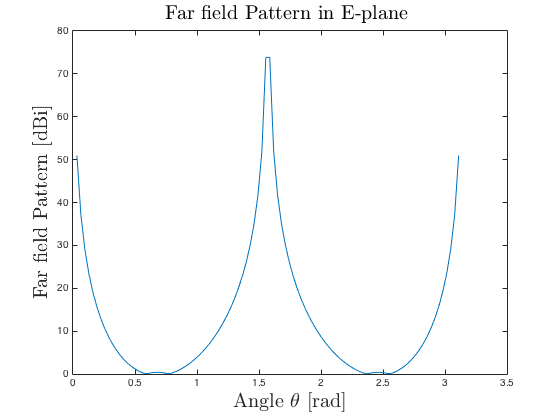
\includegraphics[scale=0.35]{/Users/marikasvensson/Documents/MATLAB/MicroProject/finished/task3/Eplane.png}
\caption{This figure shows the radiation pattern in the E-plane}
\label{task3:E-plane}
\end{figure}

\column{.5\textwidth} 
\begin{figure}[h]
\centering
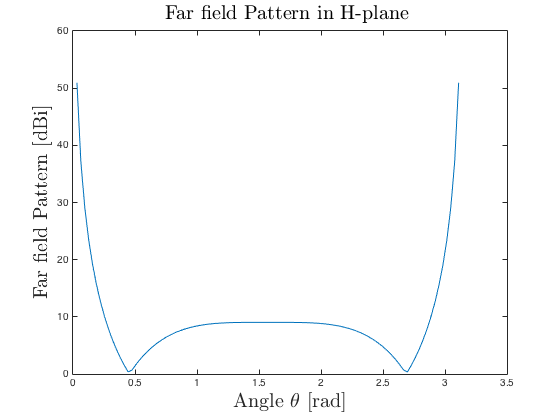
\includegraphics[scale=0.35]{/Users/marikasvensson/Documents/MATLAB/MicroProject/finished/task3/Hplane.png}
\caption{This figure shows the radiation pattern in the H-plane}
\label{task3:H-plane}
\end{figure}

\end{columns}
\end{frame}


\begin{frame}
\frametitle{Task 3: Results}
\begin{columns}[c]
\column{.45\textwidth}

\begin{figure}[h]
\centering
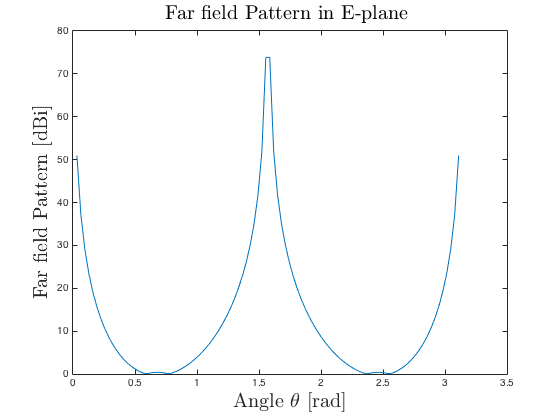
\includegraphics[scale=0.3]{/Users/marikasvensson/Documents/MATLAB/MicroProject/finished/task3/Eplane.png}
\caption{This figure shows the radiation pattern in the E-plane}
\label{task3:E-plane}
\end{figure}

\column{.5\textwidth} % Right column and width
\begin{figure}[h]
\centering
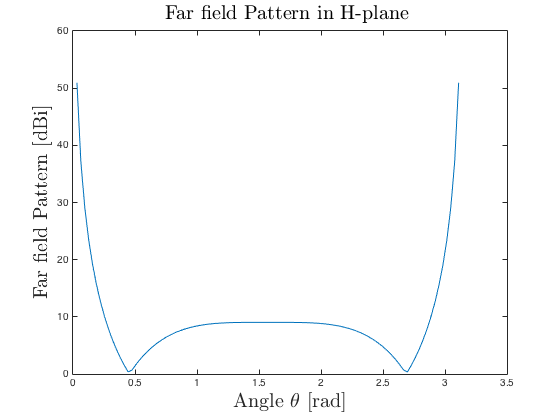
\includegraphics[scale=0.3]{/Users/marikasvensson/Documents/MATLAB/MicroProject/finished/task3/Hplane.png}
\caption{This figure shows the radiation pattern in the H-plane}
\label{task3:H-plane}
\end{figure}

\end{columns}

\end{frame}
\begin{frame}
\frametitle{Task 4: Theory}
The excitation current 
\begin{equation}
\mathbf{I} =[A_1e^{j\Phi_1} A_2e^{j\Phi_2} \dots A_{N-1}e^{j\Phi_{N-1}}],
\end{equation}
 element positions $\{\mathbf{r}_i\}_{i=1}^N$

Far field function of the array (assuming identical elements)


\begin{equation}
\mathbf{G}_A(\theta, \phi) = \sum_{n=1}^N A_ne^{j\phi_n}(G_{\theta}\hat{\theta} + G_{\phi}\hat{\phi}) e^{jk\mathbf{r}_n\dot{\hat{r}}}.
\end{equation}
Which can be written as 
\begin{equation}
\mathbf{G}_A(\theta, \phi) = \mathbf{G}(\theta, \phi) \cdot AF
\end{equation}


\end{frame}



\begin{frame}
\frametitle{Task 4: Results}
\begin{figure}[h]
\centering
\includegraphics[scale=0.3]{/Users/marikasvensson/Documents/MATLAB/MicroProject/finished/task4/Gth.png}
\caption{This figure shows $G_\theta$ as a function of $\theta$ and $\phi$}
\label{task4:Gth}
\end{figure}




\end{frame}


\begin{frame}
\frametitle{Task 4: Results}
\begin{figure}[h]
\centering
\includegraphics[scale=0.3]{/Users/marikasvensson/Documents/MATLAB/MicroProject/finished/task4/Gphi.png}
\caption{This figure shows $G_\phi$ as a function of $\theta$ and $\phi$}
\label{task4:Gphi}
\end{figure}


\end{frame}
\begin{frame}
\frametitle{Task 5: Theory}
Consider now the spherical coordinates 
\begin{equation}
\hat{r} = sin\theta cos\phi \hat{x} + sin\theta sin\phi \hat{y} + cos\theta \hat{z},
\end{equation}

\begin{align}
& d_n = \mathbf{r}_n \cdot \hat{r} = (x_n\hat{x}+ y_n\hat{y} + z_n\hat{z}) (sin\theta cos\phi \hat{x} + sin\theta sin\phi \hat{y} + cos\theta \hat{z})= \\
& sin\theta_0 cos\phi_0 x_n + sin\theta_0 sin\phi_0 y_n + cos\theta_0 z_n.
\end{align}

\begin{equation}
\Psi_{n, 0} = kd_{n,0} = \frac{2\pi}{\lambda} | sin\theta_0 cos\phi_0 (x_n) + sin\theta_0 sin\phi_0 (y_n)  + cos\theta_0 (z_n)|. 
\end{equation}

Amplitude of current was set to 1 A
\end{frame}



\begin{frame}
\frametitle{Task 5: Results}
\begin{columns}[c]
\column{.45\textwidth}
\begin{figure}[h]
\centering
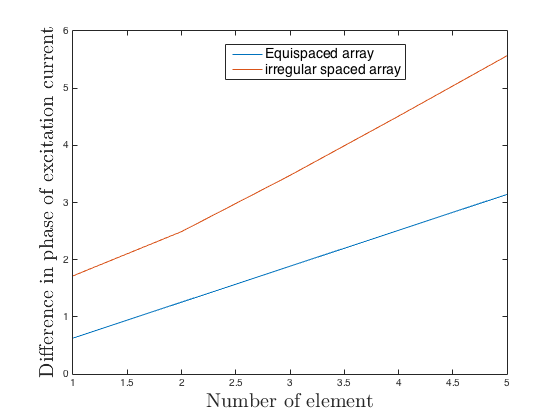
\includegraphics[scale=0.3]{/Users/marikasvensson/Documents/MATLAB/MicroProject/finished/task5/excitationCurrent.png}
\caption{This figure shows the phase of the excitation current as a function of element positions and steering direction $\theta_0 = \pi/3$rad and $\phi_0 = \pi/2$rad }
\label{task5:phase}
\end{figure}

\column{.5\textwidth} 
\begin{figure}[h]
\centering
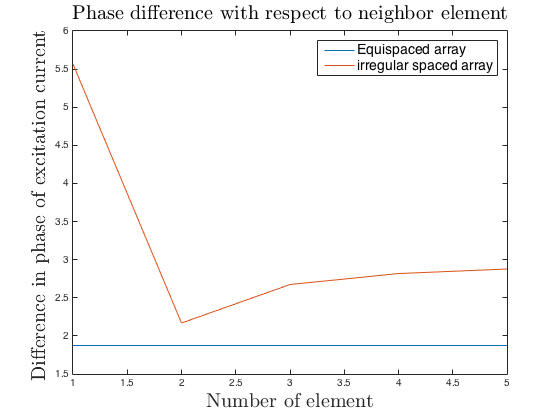
\includegraphics[scale=0.3]{/Users/marikasvensson/Documents/MATLAB/MicroProject/finished/task5/excitationCurrentNeighbour.png}
\caption{This figure shows the phase of the excitation current with respect to the neighbor as a function of element positions and steering direction $\theta_0 = \pi/3$rad and $\phi_0 = \pi/2$rad }
\label{task5:phaseNeigh}
\end{figure}
\end{columns}
\end{frame}


\begin{frame}
\frametitle{Task 6: Theory}
\begin{equation}
Pattern_{radiation}^{tot} = (\text{element radiation pattern})\times(AF)
\end{equation}
\begin{align}
& AF =  1 + e^{j(kd\cdot 1 cos(\theta) +\alpha)}  + ... + e^{j\cdot(N-1)(kdcos(\theta) +\alpha)}= \\
& e^{j(N-1)\Psi/2}sin(N\Psi/2)/ sin(\Psi/2) \Rightarrow |AF| = sin(N\Psi/2)/( N sin(\Psi/2) )
\end{align}
with $\Psi = \alpha + kdcos\theta$.  Element Pattern of horizontal dipole
\begin{equation}
f = \sqrt{1-sin(\theta)cos(\phi)}
\end{equation}


\begin{equation}
|AF|_{max} =AF(\Psi =0) \Rightarrow \alpha = kdcos(\theta_0)
\end{equation}

$\theta_0$ is called the steering angle.

H-plane: $\alpha = kdcos(\theta_0) =kd$,
Broadside :  $\alpha =0$
\end{frame}


\begin{frame}
\frametitle{Task 6a: Results}
\begin{columns}[c]



\column{.45\textwidth}

\begin{figure}[h]
\centering
\includegraphics[scale=0.3]{/Users/marikasvensson/Documents/MATLAB/MicroProject/finished/task6/6a/ypolAF.png}
\caption{This figure shows $|AF|$ as a function of $\theta$ for y polarized dipoles}
\label{task6a:ypolAF}
\end{figure}


\column{.5\textwidth} % Right column and width
\begin{figure}[h]
\centering
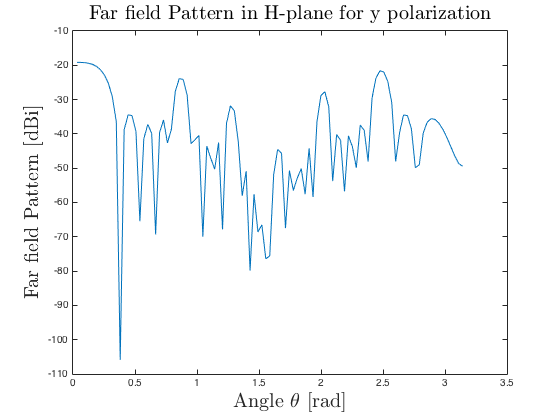
\includegraphics[scale=0.3]{/Users/marikasvensson/Documents/MATLAB/MicroProject/finished/task6/6a/ypolHplanePattern.png}
\caption{This figure shows the far field pattern as a function of $\theta$in the H-plane}
\label{task6a:ypol}
\end{figure}
\end{columns}

\end{frame}







\begin{frame}
\frametitle{Task 6b: Results}
\begin{figure}[h]
\centering
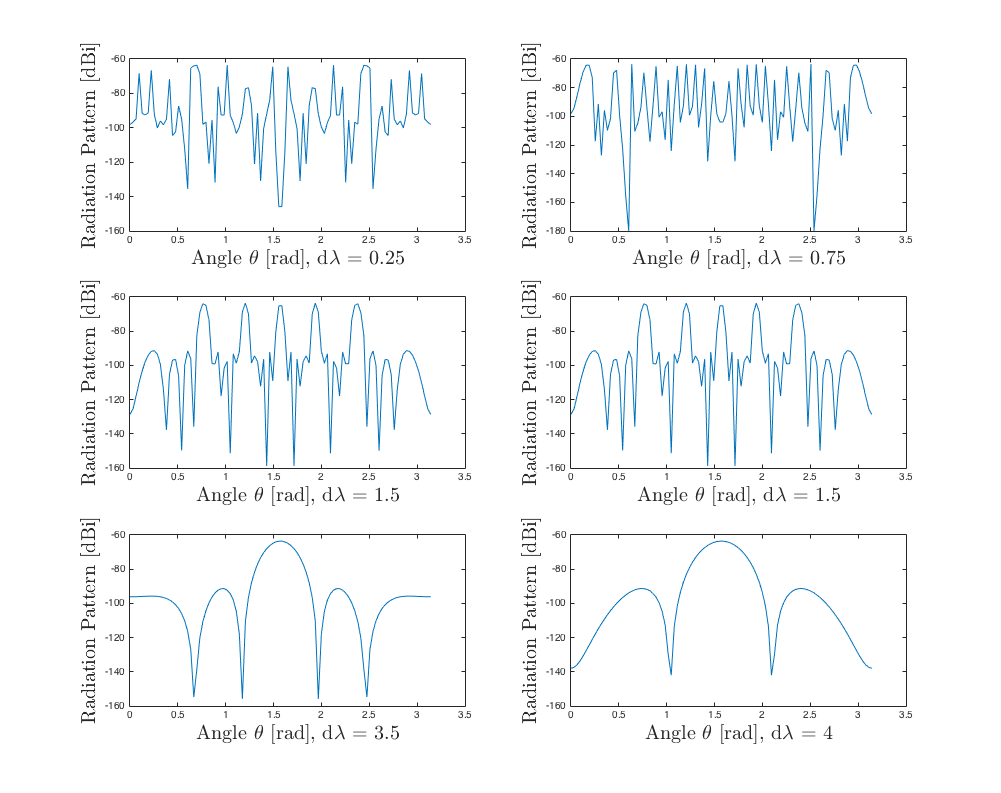
\includegraphics[scale=0.2]{/Users/marikasvensson/Documents/MATLAB/MicroProject/finished/task6/6b/ypolbroad.png}
\caption{This figure shows the far field pattern as a function of $\theta$ for y polarized dipoles in arrays}
\label{task6b:ypol}
\end{figure}
\end{frame}


\begin{frame}
\begin{figure}[h]
\centering
\includegraphics[scale=0.2]{/Users/marikasvensson/Documents/MATLAB/MicroProject/finished/task6/6b/ypolAF.png}
\caption{This figure shows $|AF|$ as a function of $\theta$ for y polarized dipoles}
\label{task6b:ypolAF}
\end{figure}
\end{frame}



\begin{frame}
\frametitle{Discussion and Conclusion}
\begin{itemize}
\item simulated results appear to recreate the theoretical expected results
\item have not found conclusive expected results for radiation patterns

\end{itemize}
\end{frame}
%------------------------------------------------



%------------------------------------------------



%------------------------------------------------
\begin{comment}
\begin{frame}
\frametitle{Blocks of Highlighted Text}
\begin{block}{Block 1}
Lorem ipsum dolor sit amet, consectetur adipiscing elit. Integer lectus nisl, ultricies in feugiat rutrum, porttitor sit amet augue. Aliquam ut tortor mauris. Sed volutpat ante purus, quis accumsan dolor.
\end{block}

\begin{block}{Block 2}
Pellentesque sed tellus purus. Class aptent taciti sociosqu ad litora torquent per conubia nostra, per inceptos himenaeos. Vestibulum quis magna at risus dictum tempor eu vitae velit.
\end{block}

\begin{block}{Block 3}
Suspendisse tincidunt sagittis gravida. Curabitur condimentum, enim sed venenatis rutrum, ipsum neque consectetur orci, sed blandit justo nisi ac lacus.
\end{block}
\end{frame}
\end{comment}
%------------------------------------------------
\begin{comment}
\begin{frame}
\frametitle{Multiple Columns}
\begin{columns}[c] % The "c" option specifies centered vertical alignment while the "t" option is used for top vertical alignment

\column{.45\textwidth} % Left column and width
\textbf{Heading}
\begin{enumerate}
\item Statement
\item Explanation
\item Example
\end{enumerate}

\column{.5\textwidth} % Right column and width
Lorem ipsum dolor sit amet, consectetur adipiscing elit. Integer lectus nisl, ultricies in feugiat rutrum, porttitor sit amet augue. Aliquam ut tortor mauris. Sed volutpat ante purus, quis accumsan dolor.

\end{columns}
\end{frame}
\end{comment}
%------------------------------------------------
\section{Discussion and Conclusion}
%------------------------------------------------
\begin{comment}
\begin{frame}
\frametitle{Table}
\begin{table}
\begin{tabular}{l l l}
\toprule
\textbf{Treatments} & \textbf{Response 1} & \textbf{Response 2}\\
\midrule
Treatment 1 & 0.0003262 & 0.562 \\
Treatment 2 & 0.0015681 & 0.910 \\
Treatment 3 & 0.0009271 & 0.296 \\
\bottomrule
\end{tabular}
\caption{Table caption}
\end{table}
\end{frame}
\end{comment}
%------------------------------------------------


%------------------------------------------------
\begin{comment}
\begin{frame}[fragile] % Need to use the fragile option when verbatim is used in the slide
\frametitle{Verbatim}
\begin{example}[Theorem Slide Code]
\begin{verbatim}
\begin{frame}
\frametitle{Theorem}
\begin{theorem}[Mass--energy equivalence]
$E = mc^2$
\end{theorem}
\end{frame}\end{verbatim}
\end{example}
\end{frame}
\end{comment}
%------------------------------------------------
\begin{comment}
\begin{frame}
\frametitle{Figure}
Uncomment the code on this slide to include your own image from the same directory as the template .TeX file.
%\begin{figure}
%\includegraphics[width=0.8\linewidth]{test}
%\end{figure}
\end{frame}
\end{comment}
%------------------------------------------------
\begin{comment}
\begin{frame}[fragile] % Need to use the fragile option when verbatim is used in the slide
\frametitle{Citation}
An example of the \verb|\cite| command to cite within the presentation:\\~

This statement requires citation \cite{p1}.
\end{frame}
\end{comment}
%------------------------------------------------
\begin{comment}
\begin{frame}
\frametitle{References}
\footnotesize{
\begin{thebibliography}{99} % Beamer does not support BibTeX so references must be inserted manually as below
\bibitem[Smith, 2012]{p1} John Smith (2012)
\newblock Title of the publication
\newblock \emph{Journal Name} 12(3), 45 -- 678.
\end{thebibliography}
}
\end{frame}
\end{comment}
%------------------------------------------------

\begin{frame}
\Huge{\centerline{Thank you for listening}}
\end{frame}

%----------------------------------------------------------------------------------------

\end{document} 